\section{Использование ПИД-регулирования с широтно-импульсной модуляцией}\label{sec:ch3/sec2}

\subsection*{Принципы реализации широтно-импульсной модуляции в пневматических системах с дискретным управлением}\label{subsec:ch3/sec2/sub1}
Широтно-импульсная модуляция (ШИМ) представляет собой метод формирования квазинепрерывного
управляющего воздействия в системах с дискретными исполнительными элементами.
В контексте пневматических систем с дискретными распределителями применение ШИМ
позволяет преодолеть ограничения, связанные с бинарным характером управления, и обеспечить более
точное регулирование положения и скорости исполнительного механизма.

Механизм формирования квазинепрерывного управляющего воздействия
посредством ШИМ основан на периодическом переключении дискретных
распределителей с определенной частотой и скважностью.

Математически это может быть описано следующим образом:

\begin{equation}
	u(t) = \begin{cases}
		1, & 0 \leq t < \alpha T; \\
		0, & \alpha T \leq t < T,
	\end{cases}
\end{equation}
где $u(t)$ -- управляющий сигнал;
$T$ -- период ШИМ;
$\alpha$ -- коэффициент заполнения $0 \leq \alpha \leq 1$.
\nomenclature{$T$}{Период ШИМ}
\nomenclature{$\alpha$}{Коэффициент заполнения\nomrefeqpage}

На рисунке \ref{fig:ch3:pwm_example} показаны временные диаграммы ШИМ-сигнала
с различными значениями коэффициента заполнения.

\begin{figure}[ht]
	\centerfloat{
		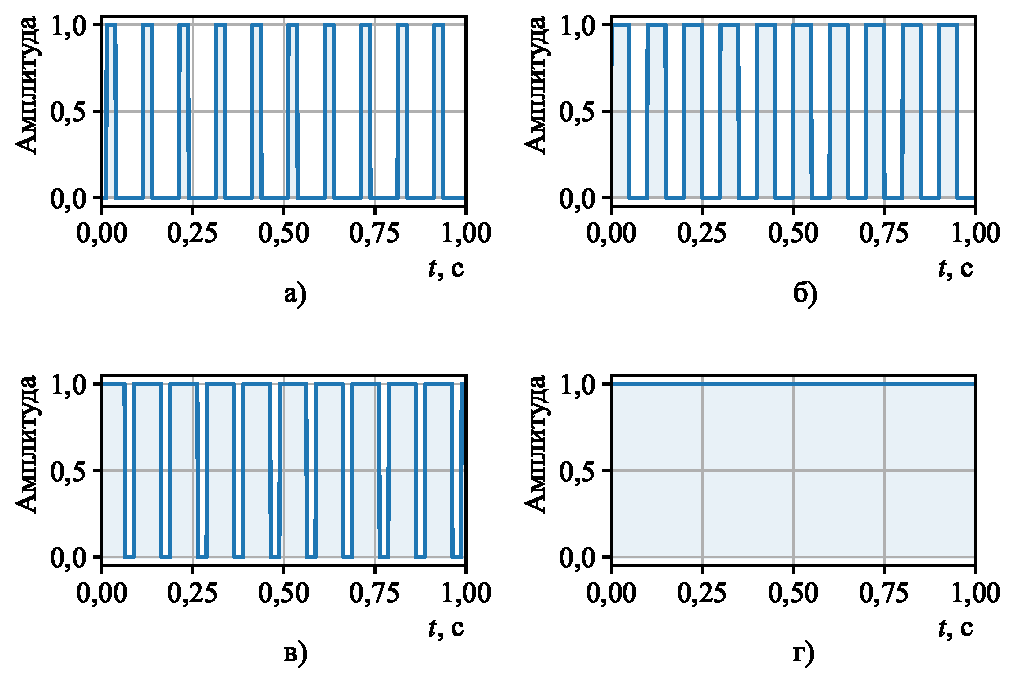
\includegraphics[]{part3/pwm_signal_skewness.pdf}
	}
	\caption{Примеры ШИМ-сигнала с различными значениями коэффициента заполнения:\\
		а) $\alpha = \num{0.3}$; б) $\alpha = \num{0.6}$; в) $\alpha = \num{0.9}$; г) $\alpha = \num{1}$}
	\label{fig:ch3:pwm_example}
\end{figure}

Среднее значение управляющего воздействия за период определяется как:
\begin{equation}
	\bar{u} = \frac{1}{T} \int_0^T u(t) dt = \alpha.
\end{equation}

Влияние частоты ШИМ на динамику пневмопривода является критическим фактором при
проектировании системы управления. С увеличением частоты ШИМ улучшается
гладкость управляющего воздействия, что способствует снижению пульсаций давления
и повышению точности позиционирования. Однако чрезмерно высокая частота может привести
к повышенному износу распределителей и увеличению энергопотребления.

Для анализа влияния частоты ШИМ на динамику системы может быть использована передаточная функция эквивалентного непрерывного звена \cite{pwm_transfer}:
\begin{equation}
	W_{\text{ШИМ}}(s) = \frac{1 - e^{-sT}}{sT},
\end{equation}
где $s$ -- комплексная переменная преобразования Лапласа.
\nomenclature{$W_{\text{ШИМ}}(s)$}{Передаточная функция ШИМ}
\nomenclature{$s$}{Комплексная переменная преобразования Лапласа\nomrefeqpage}
Особенности применения ШИМ для различных типов дискретных
распределителей обусловлены их конструктивными характеристиками и
динамическими свойствами. На рисунке \ref{fig:ch3:pwm_valve_response} показаны рассчитанные
характеристики переходных процессов для распределителя с временем срабатывания $\tau = 30$~мс и различной
частотой ШИМ сигнала.

\begin{figure}[ht]
	\centering
	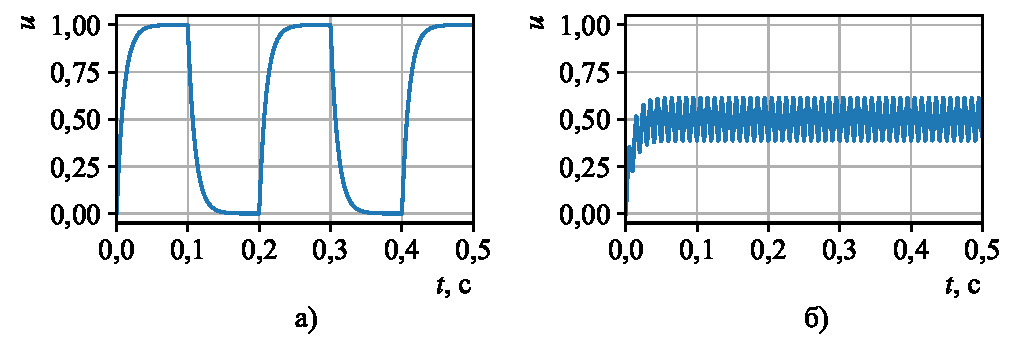
\includegraphics[]{part3/pwm_signal_transfer_function.pdf}
	\caption{Характеристики переходных процессов при различной частоте ШИМ:\\
		а) $f_{\text{ШИМ}} = \num{5}$~Гц; б) $f_{\text{ШИМ}} = \num{100}$~Гц
	}
	\label{fig:ch3:pwm_valve_response}
\end{figure}

При выборе параметров ШИМ необходимо учитывать соотношение между
периодом ШИМ и динамическими характеристиками распределителя:
\begin{equation}
	T_{ШИМ} \geq k\tau_{\text{р}},
\end{equation}
где $\tau_{\text{р}}$ -- время реакции распределителя;
$k$ -- коэффициент запаса (обычно $k \geq 2$).
\nomenclature{$\tau_{\text{р}}$}{Время реакции распределителя\nomrefeqpage}
\nomenclature{$k$}{Коэффициент запаса\nomrefeqpage}

\subsection*{Реализация ПИД-регулирования для пневмоприводов с дискретными распределителями}\label{subsec:ch3/sec2/sub2}

Применение ШИМ в пневмоприводах с дискретными распределителями открывает
возможность использования алгоритмов управления,
изначально разработанных для непрерывных систем.
Одним из наиболее эффективных и широко применяемых методов является
пропорционально-интегрально-дифференциальное (ПИД) регулирование.

Структура ПИД-регулятора для пневмопривода
с дискретными распределителями представлена на рисунке \ref{fig:ch3:pid_pwm_control}.

\begin{figure}[ht]
	\centering
	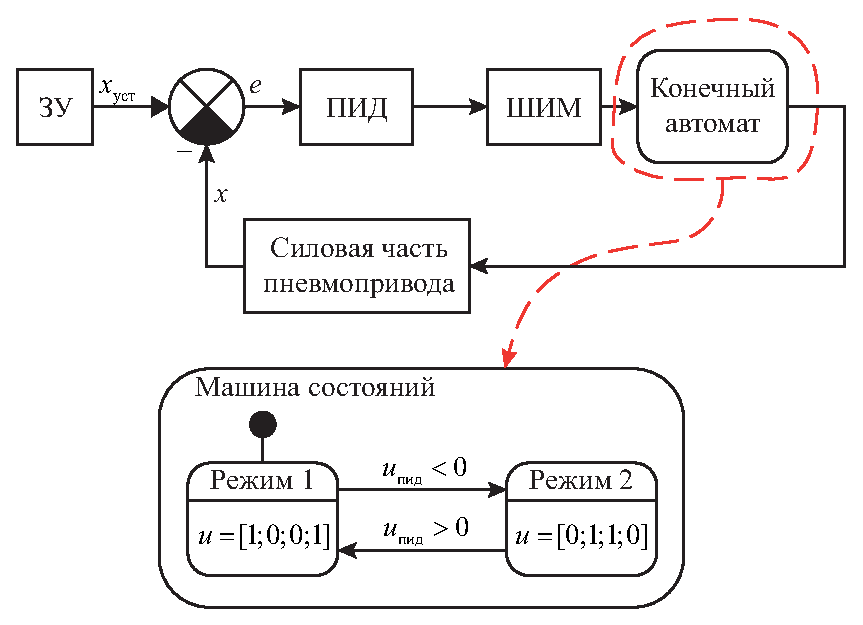
\includegraphics[]{part3/pid_pwm.eps}
	\caption{Структурная схема ПИД-регулятора с ШИМ управлением}
	\label{fig:ch3:pid_pwm_control}
\end{figure}

В данной схеме выходной сигнал ПИД-регулятора преобразуется в коэффициент
заполнения ШИМ, который управляет дискретными распределителями
пневмопривода. Этот подход позволяет достичь высокой точности
управления, характерной для непрерывных систем, в условиях
дискретного исполнительного механизма.

Математическая модель ПИД-регулятора в непрерывной форме описывается уравнением \cite{pid_pwm}:
\begin{equation}\label{eq:pid_base}
	u_{\text{пид}}(t) = K_{\text{п}} e(t) + K_{\text{и}} \int_0^t e(\tau)d\tau + K_{\text{д}}\frac{de(t)}{dt},
\end{equation}
где
$e(t)$ -- ошибка регулирования;
$K_\text{п}$, $K_\text{и}$, $K_\text{д}$ -- коэффициенты пропорциональной, интегральной и
дифференциальной составляющих соответственно;
\nomenclature{$K_\text{п}$}{Коэффициент пропорциональной составляющей\nomrefeqpage}
\nomenclature{$K_\text{и}$}{Коэффициент интегральной составляющей\nomrefeqpage}
\nomenclature{$K_\text{д}$}{Коэффициент дифференциальной составляющей\nomrefeqpage}
\nomenclature{$e(t)$}{Ошибка регулирования}

Выходной сигнал ПИД-регулятора преобразуется в коэффициент заполнения ШИМ согласно формуле:
\begin{equation}
	\alpha = \frac{u(i) + u_{max}}{2u_{max}},
\end{equation}
где $u_{max}$ -- максимальное значение управляющего сигнала.
\nomenclature{$\alpha$}{Коэффициент заполнения ШИМ\nomrefeqpage}
\nomenclature{$u_{max}$}{Максимальное значение управляющего сигнала\nomrefeqpage}

Однако в рассматриваемой конфигурации пневмопривода с дискретными распределителями
выходной сигнал ПИД-регулятора, как сказано выше, преобразуется в бинарное
управляющее воздействие посредством ШИМ. При этом возможна реализация
только двух основных режимов движения: выдвижение штока и его втягивание.

Математически это может быть описано следующим образом:

\begin{equation}
	\mathbf{u}(t) = \begin{cases}
		[1,0,0,1], & \text{если } u_\text{пид}(t) > 0; \\
		[0,1,1,0], & \text{если } u_\text{пид}(t) < 0,
	\end{cases}
\end{equation}
где $u_\text{пид}(t)$ -- выходной сигнал ПИД-регулятора.
\nomenclature{$u_\text{пид}(t)$}{Выходной сигнал ПИД-регулятора\nomrefeqpage}

Для данного случая, выходной сигнал ПИД-регулятора
преобразуется в коэффициент заполнения ШИМ согласно формуле:

\begin{equation}
	\alpha = \begin{cases}
		\frac{u_\text{ПИД}(t)}{u_{max}},  & \text{если } u_\text{ПИД}(t) > 0; \\
		-\frac{u_\text{ПИД}(t)}{u_{max}}, & \text{если } u_\text{ПИД}(t) < 0,
	\end{cases}
\end{equation}
где $u_{max}$ -- максимальное значение управляющего сигнала.

Проанализированные в дальнейших главах переходные процессы при изменении различных
параметров, и эти исследования показали, что в широком диапазоне
изменения параметров переходный процесс носит колебательный характер. В основном это связано с
тем, что при использовании ШИМ рассматривается только два состояния: выдвижение и втягивание.
В результате этого возникает резкое изменение давления в камерах распределителя, что приводит к возникновению
колебаний в системе. Данное ограничение является одной из ключевых причин для рассмотрения модифицированных
структур управления, способных обеспечить более эффективное торможение и позиционирование
привода за счет использования дополнительных режимов работы распределителей или реализации
торможения.

\subsection*{Модифицированная структура ПИД-регулятора}\label{subsec:ch3/sec2/sub3}

Как было показано выше, классическая структура ПИД-регулятора с ШИМ управлением имеет
существенные ограничения в обеспечении эффективного управления пневмоприводом с
дискретными распределителями. Основным недостатком является отсутствие прямого управления режимом торможения,
что приводит к значительному перерегулированию и колебательности системы. Для преодоления данных ограничений
предлагается модифицированная структура ПИД-регулятора, обеспечивающая адаптивное торможение на основе анализа динамического состояния системы.

Предложенная модификация базируется на концепции прогнозирования тормозного пути и формировании упреждающего
управляющего воздействия. Математическая модель модифицированного ПИД-регулятора включает три основных компонента:
классический ПИД-регулятор, описанный выражением \eqref{eq:pid_base}, блок прогнозирования тормозного пути и блок формирования тормозного воздействия.

Прогнозирование тормозного пути осуществляется на основе анализа кинетической энергии системы и желаемого ускорения торможения:

\begin{equation}\label{eq:braking_prediction}
	s_{\text{торм}}(t) = \frac{v(t)|v(t)|}{2a_{\text{торм}}} + \frac{K_{\text{б}}v(t)^2}{2},
\end{equation}
где $v(t)$ -- текущая скорость привода;
$a_{\text{торм}}$ -- желаемое ускорение торможения;
$K_{\text{б}}$ -- коэффициент запаса по тормозному пути, учитывающий инерционность пневматической системы.
\nomenclature{$s_{\text{торм}}(t)$}{Прогнозируемое тормозное расстояние\nomrefeqpage}
\nomenclature{$a_{\text{торм}}$}{Желаемое ускорение торможения\nomrefeqpage}
\nomenclature{$K_{\text{б}}$}{Коэффициент запаса по тормозному пути\nomrefeqpage}


Для учета нелинейных свойств пневматической системы в расчете тормозного пути вводится дополнительный экспоненциальный множитель:

\begin{equation}\label{eq:modified_braking_distance}
	s_{\text{торм}}(t) = \frac{v(t)|v(t)|}{2a_{\text{торм}}} \cdot \left(1 + K_\text{нл} \cdot e^{-\frac{|v(t)|}{v_\text{хар}}}\right),
\end{equation}
где $K_\text{нл}$ -- коэффициент нелинейности;
$v_\text{хар}$ -- характерная скорость, определяющая влияние нелинейности.
\nomenclature{$K_\text{нл}$}{Коэффициент нелинейности\nomrefeqpage}
\nomenclature{$v_\text{хар}$}{Характерная скорость\nomrefeqpage}

Эффективность торможения определяется соотношением между прогнозируемым
тормозным путем и расстоянием до целевой точки. Коэффициент интенсивности торможения вычисляется с использованием нелинейной функции:

\begin{equation}\label{eq:braking_intensity_expanded}
	k_{\text{торм}}(t) = \begin{cases}
		\left(1 - \min\left(\frac{s_{\text{цель}}(t)}{s_{\text{торм}}(t) \cdot k_{\text{порог}}}, 1\right)\right)^2 \cdot \eta(v), & |v(t)| > v_{\text{порог}};   \\
		0,                                                                                                                         & |v(t)| \leq v_{\text{порог}},
	\end{cases}
\end{equation}
где $s_{\text{цель}}(t) = |x_{\text{зад}} - x(t)|$ -- расстояние до целевой точки;
$k_{\text{порог}}$ -- пороговый коэффициент начала торможения;
$\eta(v)$ -- функция модуляции интенсивности торможения:

\begin{equation}\label{eq:modulation_function}
	\eta(v) = 1 - \exp\left(-\left(\frac{|v(t)|}{v_{\text{хар}}}\right)^2\right),
\end{equation}
где $v_{\text{хар}}$ -- характерная скорость, определяющая форму функции модуляции.
\nomenclature{$\eta(v)$}{Функция модуляции интенсивности торможения\nomrefeqpage}

В практической реализации для обеспечения более плавного перехода к режиму торможения и выхода из него применяется сигмоидальная функция:

\begin{equation}\label{eq:sigmoid_braking}
	k_{\text{торм}}(t) = \frac{1}{1 + e^{5\left(\frac{s_{\text{цель}}(t)}{s_{\text{торм}}(t) \cdot k_{\text{порог}}} - 0.5\right)}}.
\end{equation}

Данная функция обеспечивает плавное нарастание интенсивности торможения при приближении к целевой позиции и снижение при удалении от нее.

Для обеспечения устойчивости переключения между режимами движения и торможения вводится гистерезисная характеристика активации торможения:

\begin{equation}\label{eq:hysteresis}
	v_{\text{порог}}(t) = v_{\text{порог}}^0 \cdot \begin{cases}
		1 + \Delta v, & \text{при переходе к торможению}; \\
		1 - \Delta v, & \text{при выходе из торможения},
	\end{cases}
\end{equation}
где $v_{\text{порог}}^0$ -- базовое пороговое значение скорости;
$\Delta v$ -- ширина гистерезиса.
\nomenclature{$v_{\text{порог}}(t)$}{Пороговое значение скорости\nomrefeqpage}
\nomenclature{$\Delta v$}{Ширина гистерезиса\nomrefeqpage}

Результирующее управляющее воздействие формируется путем
взвешенной комбинации сигналов ПИД-регулятора и тормозного контура:

\begin{equation}\label{eq:combined_control}
	u_{\text{м}}(t) = (1 - k_{\text{торм}}(t))u_{\text{пид}}(t) + k_{\text{торм}}(t)u_{\text{торм}}(t),
\end{equation}
где $u_{\text{торм}}(t)$ -- сигнал управления в режиме торможения, определяемый направлением движения:
\nomenclature{$u_{\text{торм}}(t)$}{Сигнал управления в режиме торможения\nomrefeqpage}

\begin{equation}\label{eq:braking_control_expanded}
	\mathbf{u}_{\text{торм}}(t) = \begin{cases}
		[0, \alpha{\text{т}}(t), \alpha_{\text{т}}(t), 0],  & v(t) > v_{\text{порог}};      \\
		[\alpha_{\text{т}}(t), 0, 0, \alpha_{\text{т}}(t)], & v(t) < -v_{\text{порог}};     \\
		[0, 0, 0, 0],                                       & |v(t)| \leq v_{\text{порог}}.
	\end{cases}
\end{equation}

Коэффициент заполнения ШИМ в режиме торможения вычисляется с учетом динамических характеристик системы:

\begin{equation}\label{eq:braking_pwm_expanded}
	\alpha_{\text{т}}(t) = k_{\text{торм}}(t) \cdot \alpha_{\text{макс}} \cdot \left(1 + K_{\text{к}}\frac{d|v(t)|}{dt}\right),
\end{equation}
где $K_{\text{к}}$ -- коэффициент коррекции, учитывающий скорость изменения модуля скорости.
\nomenclature{$K_{\text{к}}$}{Коэффициент коррекции\nomrefeqpage}

Для повышения устойчивости системы к колебаниям при малых скоростях вблизи целевой позиции
реализовано активное демпфирование. Логика активного демпфирования заключается в формировании
управляющего воздействия, противодействующего текущему направлению движения:

\begin{equation}\label{eq:active_damping}
	\mathbf{u}_{\text{демп}}(t) = \begin{cases}
		[0, \alpha_{\text{д}}(t), 0, 0], & v(t) > 0;                     \\
		[0, 0, \alpha_{\text{д}}(t), 0], & v(t) < 0;                     \\
		[\alpha_{\text{д}}(t), 0, 0, 0], & v(t) = 0 \text{ и } e(t) > 0; \\
		[0, 0, 0, \alpha_{\text{д}}(t)], & v(t) = 0 \text{ и } e(t) < 0,
	\end{cases}
\end{equation}
где $\alpha_{\text{д}}(t) = K_{\text{д}} \cdot |v(t)| \cdot \alpha_{\text{макс}}$ -- коэффициент заполнения ШИМ для демпфирования;
$K_{\text{д}}$ -- коэффициент демпфирования;
$e(t)$ -- ошибка позиционирования.

Дополнительно в модифицированной структуре ПИД-регулятора реализован механизм защиты от
интегрального насыщения, который адаптивно ограничивает скорость нарастания
интегральной составляющей при насыщении управляющего сигнала:

\begin{equation}\label{eq:anti_windup}
	I(t) = \begin{cases}
		I(t-1) + K_{\text{и}} \cdot e(t) \cdot \Delta t \cdot \gamma, & \text{при насыщении};  \\
		I(t-1) + K_{\text{и}} \cdot e(t) \cdot \Delta t,              & \text{в иных случаях},
	\end{cases}
\end{equation}
где $I(t)$ -- интегральная составляющая;
$\gamma$ -- коэффициент снижения скорости интегрирования ($\gamma < 1$);
$\Delta t$ -- интервал дискретизации.
\nomenclature{$\gamma$}{Коэффициент снижения скорости интегрирования\nomrefeqpage}
\nomenclature{$\Delta t$}{Интервал дискретизации\nomrefeqpage}

Для фильтрации высокочастотных шумов в дифференциальной составляющей применяется экспоненциальный фильтр:

\begin{equation}\label{eq:derivative_filter}
	D(t) = \alpha \cdot \frac{e(t) - e(t-1)}{\Delta t} + (1-\alpha) \cdot D(t-1),
\end{equation}
где $D(t)$ -- отфильтрованная дифференциальная составляющая;
$\alpha$ -- коэффициент фильтрации ($0 < \alpha < 1$).
\nomenclature{$\alpha$}{Коэффициент фильтрации\nomrefeqpage}

Данный алгоритм был зарегистрирован в качестве программы для ЭВМ \cite{progbib1}.

Исследование динамических характеристик системы управления электропневматическим приводом демонстрирует существенные различия в характере
переходных процессов для классической и модифицированной структур ПИД-регулятора с ШИМ.

Для классической структуры характерно наличие значительной колебательности, обусловленной отсутствием эффективного
управления торможением. Это проявляется в перерегулировании при подходе к заданной позиции и возникновении затухающих или авто-колебаний
из-за ограниченности режимов работы распределителей.

Модифицированная структура обеспечивает более качественный переходный процесс благодаря адаптивному торможению и
прогнозированию тормозного пути.

\begin{figure}
	\centering
	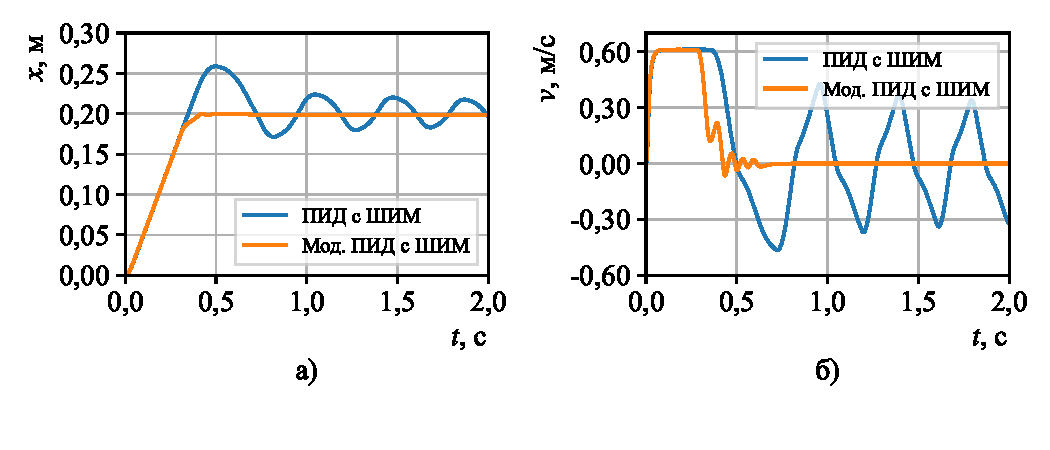
\includegraphics[]{part3/pid_comparison_2.pdf}
	\caption{Сравнение переходных процессов для классической и модифицированной структур ПИД-регулятора с ШИМ управлением:\\
		а) позиционирование штока; б) скорость штока}
	\label{fig:ch3:transient_comparison}
\end{figure}

Представленные на рисунке \ref{fig:ch3:transient_comparison} результаты наглядно демонстрируют преимущества
модифицированной структуры в обеспечении качества позиционирования пневмопривода. Предложенная структура
позволяет существенно снизить колебательность процесса и устранить перерегулирование при сохранении приемлемой статической точности позиционирования.
Внедрение механизмов прогнозирования тормозного пути, активного демпфирования и защиты от интегрального насыщения обеспечивает
робастность системы к параметрическим возмущениям и изменениям динамических характеристик пневмопривода.
